\chapter{Schedules}
\label{chap:introduction-schedules}

We will now combine the knowledge from chapter \ref{chap:theoretical-foundations} and introduce the problem we will be working on. 

\section{Computational setting}
\label{sec:schedules-problem-setting}

We now describe our assumptions concerning the tasks to be processed and our machines.

\paragraph{Intree constraint}

We assume that the dependencies between the tasks under consideration can be described as an intree (as introduced in  section \ref{sec:foundations-graph-theory}).

\paragraph{Random task processing times}

We assume that we do not know the processing time for a certain task in advance. We instead assume that we can model the task time for each task within the intree by an exponentially distributed random variable as defined in section \ref{sec:exponential-distribution}. We furthermore assume that all tasks are exponentially distributed with the \emph{same} parameter $\lambda$. Note that we can assume w.l.o.g. --  according to theorem \ref{thm:expoenential-distr-scalability} explaining exponential variables' scaling -- that all tasks have parameter $\lambda=1$.

\paragraph{Parallel processors}

We assume that we have a certain number (we will focus on 2 or 3) of \emph{identical} processors. These processors work in parallel and can be used to carry out the individual tasks. For simplicity we assume that switching from one task to another takes no time at all.

\paragraph{Tasks are ``atomic''}

We assume that one single task can be processed by one processor exclusively, i.e. it is not possible to save time by ``splitting'' one single task over several processors. That, moreover, means that there might be idle processors if we have more ready tasks than processors.

\paragraph{Non-preemtive scheduling}

We will focus on non-preemtive scheduling, i.e. once a task is processor is assigned a task, this task has to be processed \emph{completely} before the processor can be used for anything else. Note that the restriction on non-preemtive scheduling is no problem when we work with two processors (as shown in \cite{chandyreynoldslargepaper1979}) --- in this case, the optimal schedule is (without loss of generality) non-preemtive. However, for three processors, preemtive schedules might be better than non-preemtive ones. We will later show an example intree for this fact (see section \ref{preemtiveness-explanation}).

However, as shown in \cite{chandyreynoldslargepaper1979} an optimal schedule (without loss of generality) only preemts a task directly after another task finishes.

\subsection{Processing a whole intree of tasks}
\label{sec:processing-an-intree-of-tasks}

Assuming that we have a certain amount $p$ of identical processors, we can process all tasks in an intree (of course in a valid order). Naturally, We have to do this step by step. 

That is, we assign some (at most $p$) ready tasks to processors, wait until the first assigned task finishes, assign a new task (if available) to the now idle processor, and continue with the subtree obtained by removing the finished task. That is, in each point of time, we know the current intree containing all tasks not yet finished and all tasks currently being processed. We therefore introduce the notation of \emph{snapshots}.

\begin{definition}[Schedules and snapshots]  
  Let $I$ be an intree of tasks that is processed. A \emph{schedule} is the order in which tasks are processed. Since task times are unknown, this order is not deterministic and can vary from execution to execution.

  Let $S$ be a schedule of $I$.
  A \emph{snapshot} of $S$ a pair containing
  \begin{itemize}
  \item the current subtree $I'\subseteq I$ describing which tasks are not finished yet,
  \item a set $X$ holding the tasks that are currently being processed (i.e. a set of \emph{currently scheduled tasks}).
  \end{itemize}
\end{definition}

While the above definition is well suited for theoretical considerations, we -- most of the time -- are satisfied with a concise graphical representation, that will look as shown in figure \ref{fig:intro-snapshot-graphical-representation}, i.e. it is depicted as an intree, whose scheduled tasks are marked drawn by a 
\tikz{\node[circle, scale=0.75, fill, task_scheduled] (tid7) at (2.25,6){};} 
while the non-scheduled tasks are drawn as
\tikz{\node[circle, scale=0.75, fill] (tid7) at (2.25,6){};}
.

\begin{figure}[t]
  \centering
  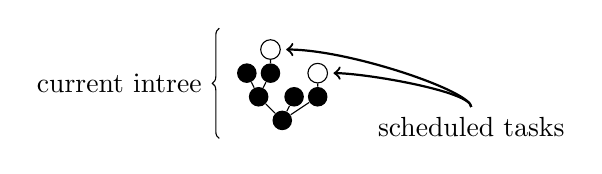
\begin{tikzpicture}[scale=.2, anchor=south]
    \node[circle, scale=0.75, fill] (tid0) at (3,1.5){};
    \node[circle, scale=0.75, fill] (tid1) at (1.5,3){};
    \node[circle, scale=0.75, fill] (tid3) at (0.75,4.5){};
    \node[circle, scale=0.75, fill] (tid4) at (2.25,4.5){};
    \node[circle, scale=0.75, fill, task_scheduled] (tid7) at (2.25,6){};
    \draw[](tid4) -- (tid7);
    \draw[](tid1) -- (tid3);
    \draw[](tid1) -- (tid4);
    \node[circle, scale=0.75, fill] (tid2) at (3.75,3){};
    \node[circle, scale=0.75, fill] (tid5) at (5.25,3){};
    \node[circle, scale=0.75, fill, task_scheduled] (tid6) at (5.25,4.5){};
    \draw[](tid5) -- (tid6);
    \draw[](tid0) -- (tid1);
    \draw[](tid0) -- (tid2);
    \draw[](tid0) -- (tid5);
    % arrows for scheduled tasks
    \draw(tid7) +(1,0)[<-, thick] ..controls+(4,0) and +(0,1).. (15,3);
    \draw(tid6) +(1,0)[<-, thick] ..controls+(2,0) and +(0,1).. (15,3) 
    node[below]{scheduled tasks};
    % brace for whole intree
    \draw[decorate, decoration=brace](-1,1) --node[left, xshift=-.1cm]{current intree} +(0,7);
  \end{tikzpicture}
  \caption{A snapshot is determined by its intree and a collection of currently scheduled tasks.}
  \label{fig:intro-snapshot-graphical-representation}
\end{figure}

Consider now a snapshot, i.e. the current intree and a set of currently scheduled tasks. At this point, there are several possibilities:

\begin{itemize}
\item Any of the currently scheduled tasks may be the first task to finish.
\item If a certain task finishes, the corresponding processor gets idle and can be assigned new work. That is, we may be able to choose a new task\footnote{It may be the case that we are not able to select any new task because all leaves are already scheduled. In this case, the processor has to stay idle and can not get assigned a new task.} and assign it to the now idle processor.

  Note that we can -- in principle -- easily choose a certain task with some probability and another task with another probability, thus introducing more possibilities.
\end{itemize}

That is, we have several possibilities here. The first of them (which task finishes first) can not be influenced in our scenario. The second, however, leaves us a choice that we can influence. Depending on which task we choose next, we might get a better or worse overall run time.

\begin{definition}[Scheduling strategy]
  A \emph{scheduling strategy} determines the probability that a certai tasks should be the next tasks to be scheduled.
\end{definition}

That means, we use the notion of a \emph{probabilistic scheduler} in the sense that the scheduler is not forced to restrict on \emph{one single} task, but can instead specify probabilities for each ready, currently unscheduled task. Note that we can easily ``simulate'' a deterministic scheduler by assigning probability 1 to one single ready task, and probability 0 to all other possibilities.

One desirable goal is to always choose the next task to be scheduled (resp. the respective probabilities) in such a way that the overall expected run time is minimal. We will now see how we can compute the expected run time for a schedule.

\subsection{Two prominent scheduling strategies}
\label{sec:intro-two-scheduling-strategies}

We will now present two important scheduling strategies that we will use to research the problem throughout this work.

\begin{definition}[HLF scheduling]
  A \emph{highest level first} scheduler (or HLF scheduler) assigns, if there are idle processors, ready tasks whose levels are maximal.
\end{definition}

Note that the above definition of HLF leaves some freedom if there are several tasks that could be chosen by HLF. If this is the case, then there are (basically) two possibilities:
\begin{itemize}
\item Choose \emph{one} task according to a certain pattern or randomly.
\item Assign to \emph{each} possibly chosen task a certain probability.
\end{itemize}

Note that we can consider the first possibility as a special case of the second one. HLF scheduling is optimal for intrees whose task times are equal scheduled on any number of processors \cite{hu:1961:hlfoptimalforknowntimesintree} and for intrees whose task times are exponentially distributed (with same parameter) scheduled on two processors (see \cite{chandyreynoldsshortpaper1975} and chapter \ref{chap:p2}). 

Another (very trivial) scheduler is the scheduler that tries all possibilities:

\begin{definition}[LEAF scheduling]
  A LEAF scheduler, if a processor gets free and can be assigned a new task, assigns each ready task with the same probability to this processor. In the beginning, each possible combination of scheduled tasks is taken with the same probability.
\end{definition}

LEAF schedulers are useful to examine all possible schedules and play an important role when we research how many snapshots have to be examined \emph{at most}. Note that a LEAF scheduler examines \emph{all possible} schedules. The resulting schedule, thus, \emph{must} contain the optimal choices as a part of it. That means, we can compute an optimal schedule by first scheduling the intree with the LEAF scheduler, and afterwards excluding the ``wrong'' (i.e. suboptimal) choices.

\section{Visualizing a schedule}
\label{sec:intro-visualizing-schedules}

If we are speaking of a schedule, we talk about the complete processing of an intree of tasks.

We can think of it as a connected directed acyclic graph or DAG (see \cite{diestel2005graph} for more information), where each vertex represents one single snapshot. The edges between the snapshots then represent transitions that indicate that a certain task has finished and (possibly) a new task has chosen to be scheduled. We can naturally assign the edges weights that represent the corresponding probability that a task has finished and the new task has been picked.

As stated before, we have two sources of non-determinism:
\begin{itemize}
\item Each of the currently scheduled tasks can be the first task to finish. Depending on which task finishes first, we have to continue with another intree.
\item When one task finishes, the corresponding processor becomes idle and can be used to process other tasks. This is the second source where we have different possibilities. However, for this point, we can decide ourselves how to continue.
\end{itemize}

We will look at the intree $(0,0,1,2,2,2,6,6,8)$ -- it shall be processed by two processors -- as an example. This intree looks as follows:

\begin{center}
  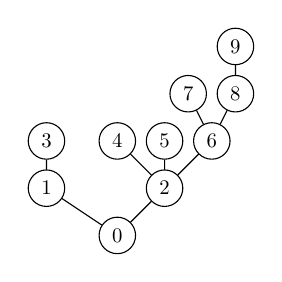
\begin{tikzpicture}[scale=.4]
    \node[circle, scale=0.75, draw] (tid0) at (4.5,1.5){0};
    \node[circle, scale=0.75, draw] (tid2) at (2.25,3){1};
    \node[circle, scale=0.75, draw] (tid4) at (2.25,4.5){3};
    \draw[](tid2) -- (tid4);
    \node[circle, scale=0.75, draw] (tid3) at (6,3){2};
    \node[circle, scale=0.75, draw] (tid5) at (4.5,4.5){4};
    \node[circle, scale=0.75, draw] (tid6) at (6,4.5){5};
    \node[circle, scale=0.75, draw] (tid7) at (7.5,4.5){6};
    \node[circle, scale=0.75, draw] (tid8) at (6.75,6){7};
    \node[circle, scale=0.75, draw] (tid9) at (8.25,6){8};
    \node[circle, scale=0.75, draw] (tid10) at (8.25,7.5){9};
    \draw[](tid9) -- (tid10);
    \draw[](tid7) -- (tid8);
    \draw[](tid7) -- (tid9);
    \draw[](tid3) -- (tid5);
    \draw[](tid3) -- (tid6);
    \draw[](tid3) -- (tid7);
    \draw[](tid0) -- (tid2);
    \draw[](tid0) -- (tid3);
  \end{tikzpicture}
\end{center}

Figure \ref{fig:schedule-dag-intro} shows (the beginning) a two-processor schedule for the intree $(0,0,1,2,2,2,6.6,8)$ in two variants: Figure \ref{fig:schedule-dag-intro-intermediates} shows the schedule and incorporates situations where the scheduler can decide wich tasks should be scheduled next with wich probabilities (``intermediate snapshots''). At the beginning, the nodes 9 and 3 are scheduled (snapshot $A$). Then each of these two tasks is the first one to finish (each one with probability 50\%). This intermediate situation, where exactly one of the two tasks is finished and the scheduler can assign probabilities describing which task to pick next, are shown in snapshots $B$ (this is the situation where task 3 finished first) and $C$ (where 9 finished first).

In the situation described by the intermediate snapshot $B$, the scheduler can decide which task shall be chosen next with which probability. In the situation of snapshot $B$, the scheduler decides that with probability 20\%, the task 1 shall be chosen as next task (snapshot $B_1$) and with probability 80\% task 4 shall be chosen as next task (snapshot $B_2$). Similarily it decides in the situation denoted by $C$ that tasks 8 resp. 4 shall be chosen with probability 40\% each ($C_1$ resp. $C_3$) and task 7 shall be chosen with probability 20\% ($C_2$).

\begin{figure}[th]
  \centering
  \begin{subfigure}{\textwidth}
    \centering
    \renewcommand{\leveltopI}{-12cm + \leveltop}
\renewcommand{\leveltopII}{-12cm + \leveltopI}
\renewcommand{\leveltopIII}{-14cm + \leveltopII}
\renewcommand{\leveltopIIII}{-12cm + \leveltopIII}
\renewcommand{\leveltopIIIII}{-12cm + \leveltopIIII}
\renewcommand{\leveltopIIIIII}{-12cm + \leveltopIIIII}
\renewcommand{\leveltopIIIIIII}{-12cm + \leveltopIIIIII}
\renewcommand{\leveltopIIIIIIII}{-12cm + \leveltopIIIIIII}
\renewcommand{\leveltopIIIIIIIII}{-12cm + \leveltopIIIIIIII}
\renewcommand{\leveltopIIIIIIIIII}{-12cm + \leveltopIIIIIIIII}
\renewcommand{\leveltopIIIIIIIIIII}{-12cm + \leveltopIIIIIIIIII}
\begin{tikzpicture}[scale=.2, anchor=south]
  % "key"
  \fill[fill=gray!10!white] (-35, -24) rectangle +(72, 9.5);
  \draw[dashed] (-35, -14.5) -- +(72, 0);
  \draw[dashed] (-35, -24) -- +(72, 0);
  \node at (27, -21) {Intermediate snapshots};
  \begin{scope}[yshift=\leveltopI cm]
    \node at (-7.5,3) {\huge $A$};
    \matrix (line1)[column sep=0.5cm] {
      \node[draw=black, rectangle split,  rectangle split parts=1] (sn0x17d67b0){
        \begin{tikzpicture}[scale=.2]
          \node[circle, scale=0.75, fill] (tid0) at (4.5,1.5){};
          \node[circle, scale=0.75, fill] (tid2) at (2.25,3){};
          \node[circle, scale=0.75, fill, task_scheduled] (tid4) at (2.25,4.5){};
          \draw[](tid2) -- (tid4);
          \node[circle, scale=0.75, fill] (tid3) at (6,3){};
          \node[circle, scale=0.75, fill] (tid5) at (3.75,4.5){};
          \node[circle, scale=0.75, fill] (tid6) at (5.25,4.5){};
          \node[circle, scale=0.75, fill] (tid7) at (7.5,4.5){};
          \node[circle, scale=0.75, fill] (tid8) at (6.75,6){};
          \node[circle, scale=0.75, fill] (tid9) at (8.25,6){};
          \node[circle, scale=0.75, fill, task_scheduled] (tid10) at (8.25,7.5){};
          \draw[](tid9) -- (tid10);
          \draw[](tid7) -- (tid8);
          \draw[](tid7) -- (tid9);
          \draw[](tid3) -- (tid5);
          \draw[](tid3) -- (tid6);
          \draw[](tid3) -- (tid7);
          \draw[](tid0) -- (tid2);
          \draw[](tid0) -- (tid3);
        \end{tikzpicture}
      };
      & 
      \\
    };
  \end{scope}
  \begin{scope}[yshift=\leveltopII cm]
    \matrix (line2)[column sep=0.5cm] {
      \node[draw=black, rectangle split,  rectangle split parts=1] (sn0x17d65a0){
        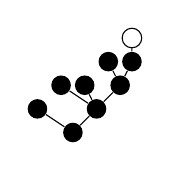
\begin{tikzpicture}[scale=.2]
          \node[circle, scale=0.75, fill] (tid0) at (4.5,1.5){};
          \node[circle, scale=0.75, fill] (tid2) at (2.25,3){};
          \node[circle, scale=0.75, fill] (tid3) at (6,3){};
          \node[circle, scale=0.75, fill] (tid5) at (3.75,4.5){};
          \node[circle, scale=0.75, fill] (tid6) at (5.25,4.5){};
          \node[circle, scale=0.75, fill] (tid7) at (7.5,4.5){};
          \node[circle, scale=0.75, fill] (tid8) at (6.75,6){};
          \node[circle, scale=0.75, fill] (tid9) at (8.25,6){};
          \node[circle, scale=0.75, fill, task_scheduled] (tid10) at (8.25,7.5){};
          \draw[](tid9) -- (tid10);
          \draw[](tid7) -- (tid8);
          \draw[](tid7) -- (tid9);
          \draw[](tid3) -- (tid5);
          \draw[](tid3) -- (tid6);
          \draw[](tid3) -- (tid7);
          \draw[](tid0) -- (tid2);
          \draw[](tid0) -- (tid3);
        \end{tikzpicture}
      }
      node[left, xshift=-25, yshift=25]{\huge $B$};
      & 
      \node[minimum width=1cm]{};
      &
      \node[draw=black, rectangle split,  rectangle split parts=1] (sn0x17d57c0){
        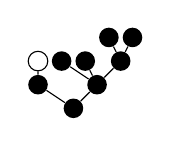
\begin{tikzpicture}[scale=.2]
          \node[circle, scale=0.75, fill] (tid0) at (4.5,1.5){};
          \node[circle, scale=0.75, fill] (tid2) at (2.25,3){};
          \node[circle, scale=0.75, fill, task_scheduled] (tid4) at (2.25,4.5){};
          \draw[](tid2) -- (tid4);
          \node[circle, scale=0.75, fill] (tid3) at (6,3){};
          \node[circle, scale=0.75, fill] (tid5) at (3.75,4.5){};
          \node[circle, scale=0.75, fill] (tid6) at (5.25,4.5){};
          \node[circle, scale=0.75, fill] (tid7) at (7.5,4.5){};
          \node[circle, scale=0.75, fill] (tid8) at (6.75,6){};
          \node[circle, scale=0.75, fill] (tid9) at (8.25,6){};
          \draw[](tid7) -- (tid8);
          \draw[](tid7) -- (tid9);
          \draw[](tid3) -- (tid5);
          \draw[](tid3) -- (tid6);
          \draw[](tid3) -- (tid7);
          \draw[](tid0) -- (tid2);
          \draw[](tid0) -- (tid3);
        \end{tikzpicture}
      }
      node[left, xshift=-25, yshift=25]{\huge $C$};
      & 
      \\
    };
  \end{scope}
  \begin{scope}[yshift=\leveltopIII cm]
    \matrix (line3)[column sep=0.5cm] {
      \node[draw=black, rectangle split,  rectangle split parts=1] (sn0x17d55b0){
        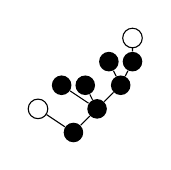
\begin{tikzpicture}[scale=.2]
          \node[circle, scale=0.75, fill] (tid0) at (4.5,1.5){};
          \node[circle, scale=0.75, fill, task_scheduled] (tid2) at (2.25,3){};
          \node[circle, scale=0.75, fill] (tid3) at (6,3){};
          \node[circle, scale=0.75, fill] (tid5) at (3.75,4.5){};
          \node[circle, scale=0.75, fill] (tid6) at (5.25,4.5){};
          \node[circle, scale=0.75, fill] (tid7) at (7.5,4.5){};
          \node[circle, scale=0.75, fill] (tid8) at (6.75,6){};
          \node[circle, scale=0.75, fill] (tid9) at (8.25,6){};
          \node[circle, scale=0.75, fill, task_scheduled] (tid10) at (8.25,7.5){};
          \draw[](tid9) -- (tid10);
          \draw[](tid7) -- (tid8);
          \draw[](tid7) -- (tid9);
          \draw[](tid3) -- (tid5);
          \draw[](tid3) -- (tid6);
          \draw[](tid3) -- (tid7);
          \draw[](tid0) -- (tid2);
          \draw[](tid0) -- (tid3);
        \end{tikzpicture}
      }
      node[left, xshift=-25, yshift=25]{\huge $B_1$};
      & 
      \node[draw=black, rectangle split,  rectangle split parts=1] (sn0x17d6160){
        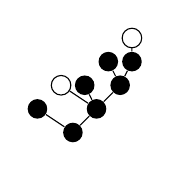
\begin{tikzpicture}[scale=.2]
          \node[circle, scale=0.75, fill] (tid0) at (4.5,1.5){};
          \node[circle, scale=0.75, fill] (tid2) at (2.25,3){};
          \node[circle, scale=0.75, fill] (tid3) at (6,3){};
          \node[circle, scale=0.75, fill, task_scheduled] (tid5) at (3.75,4.5){};
          \node[circle, scale=0.75, fill] (tid6) at (5.25,4.5){};
          \node[circle, scale=0.75, fill] (tid7) at (7.5,4.5){};
          \node[circle, scale=0.75, fill] (tid8) at (6.75,6){};
          \node[circle, scale=0.75, fill] (tid9) at (8.25,6){};
          \node[circle, scale=0.75, fill, task_scheduled] (tid10) at (8.25,7.5){};
          \draw[](tid9) -- (tid10);
          \draw[](tid7) -- (tid8);
          \draw[](tid7) -- (tid9);
          \draw[](tid3) -- (tid5);
          \draw[](tid3) -- (tid6);
          \draw[](tid3) -- (tid7);
          \draw[](tid0) -- (tid2);
          \draw[](tid0) -- (tid3);
        \end{tikzpicture}
      }
      node[left, xshift=-25, yshift=25]{\huge $B_2$};
      & 
      \node[draw=black, rectangle split,  rectangle split parts=1] (sn0x17d5380){
        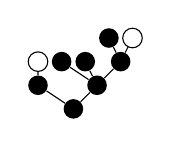
\begin{tikzpicture}[scale=.2]
          \node[circle, scale=0.75, fill] (tid0) at (4.5,1.5){};
          \node[circle, scale=0.75, fill] (tid2) at (2.25,3){};
          \node[circle, scale=0.75, fill, task_scheduled] (tid4) at (2.25,4.5){};
          \draw[](tid2) -- (tid4);
          \node[circle, scale=0.75, fill] (tid3) at (6,3){};
          \node[circle, scale=0.75, fill] (tid5) at (3.75,4.5){};
          \node[circle, scale=0.75, fill] (tid6) at (5.25,4.5){};
          \node[circle, scale=0.75, fill] (tid7) at (7.5,4.5){};
          \node[circle, scale=0.75, fill] (tid8) at (6.75,6){};
          \node[circle, scale=0.75, fill, task_scheduled] (tid9) at (8.25,6){};
          \draw[](tid7) -- (tid8);
          \draw[](tid7) -- (tid9);
          \draw[](tid3) -- (tid5);
          \draw[](tid3) -- (tid6);
          \draw[](tid3) -- (tid7);
          \draw[](tid0) -- (tid2);
          \draw[](tid0) -- (tid3);
        \end{tikzpicture}
      }
      node[left, xshift=-25, yshift=25]{\huge $C_1$};
      & 
      \node[draw=black, rectangle split,  rectangle split parts=1] (sn0x17d2f50){
        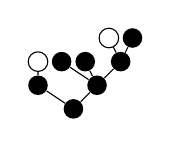
\begin{tikzpicture}[scale=.2]
          \node[circle, scale=0.75, fill] (tid0) at (4.5,1.5){};
          \node[circle, scale=0.75, fill] (tid2) at (2.25,3){};
          \node[circle, scale=0.75, fill, task_scheduled] (tid4) at (2.25,4.5){};
          \draw[](tid2) -- (tid4);
          \node[circle, scale=0.75, fill] (tid3) at (6,3){};
          \node[circle, scale=0.75, fill] (tid5) at (3.75,4.5){};
          \node[circle, scale=0.75, fill] (tid6) at (5.25,4.5){};
          \node[circle, scale=0.75, fill] (tid7) at (7.5,4.5){};
          \node[circle, scale=0.75, fill, task_scheduled] (tid8) at (6.75,6){};
          \node[circle, scale=0.75, fill] (tid9) at (8.25,6){};
          \draw[](tid7) -- (tid8);
          \draw[](tid7) -- (tid9);
          \draw[](tid3) -- (tid5);
          \draw[](tid3) -- (tid6);
          \draw[](tid3) -- (tid7);
          \draw[](tid0) -- (tid2);
          \draw[](tid0) -- (tid3);
        \end{tikzpicture}
      }
      node[left, xshift=-25, yshift=25]{\huge $C_2$};
      & 
      \node[draw=black, rectangle split,  rectangle split parts=1] (sn0x17d3a00){
        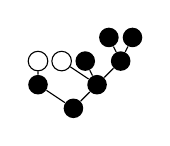
\begin{tikzpicture}[scale=.2]
          \node[circle, scale=0.75, fill] (tid0) at (4.5,1.5){};
          \node[circle, scale=0.75, fill] (tid2) at (2.25,3){};
          \node[circle, scale=0.75, fill, task_scheduled] (tid4) at (2.25,4.5){};
          \draw[](tid2) -- (tid4);
          \node[circle, scale=0.75, fill] (tid3) at (6,3){};
          \node[circle, scale=0.75, fill, task_scheduled] (tid5) at (3.75,4.5){};
          \node[circle, scale=0.75, fill] (tid6) at (5.25,4.5){};
          \node[circle, scale=0.75, fill] (tid7) at (7.5,4.5){};
          \node[circle, scale=0.75, fill] (tid8) at (6.75,6){};
          \node[circle, scale=0.75, fill] (tid9) at (8.25,6){};
          \draw[](tid7) -- (tid8);
          \draw[](tid7) -- (tid9);
          \draw[](tid3) -- (tid5);
          \draw[](tid3) -- (tid6);
          \draw[](tid3) -- (tid7);
          \draw[](tid0) -- (tid2);
          \draw[](tid0) -- (tid3);
        \end{tikzpicture}
      }
      node[left, xshift=-25, yshift=25]{\huge $C_3$};
      & 
      \\
    };
  \end{scope}
  \draw (sn0x17d67b0.south) -- node[xshift=.4cm]{$0.5$} (sn0x17d57c0.north);
  \draw (sn0x17d67b0.south) -- node[left, xshift=-.4cm]{$0.5$} (sn0x17d65a0.north);
  \draw (sn0x17d65a0.south) -- node[right, xshift=.25cm]{$0.8$} (sn0x17d6160.north);
  \draw (sn0x17d65a0.south) -- node[left, xshift=-.25cm]{$0.2$} (sn0x17d55b0.north);
  \draw (sn0x17d57c0.south) -- node[right, xshift=.25]{$0.2$} (sn0x17d2f50.north);
  \draw (sn0x17d57c0.south) -- node[xshift=-.5]{$0.4$} (sn0x17d5380.north);
  \draw (sn0x17d57c0.south) -- node[right, xshift=.25]{$0.4$} (sn0x17d3a00.north);
\end{tikzpicture}
%%% Local Variables:
%%% TeX-master: "thesis/thesis.tex"
%%% End: 

    \caption{A snapshot DAG with intermediate snapshots. In the beginning, there are two tasks scheduled. Each task is the first to finish with probability 0.5 (see the corresponding edges). An intermediate snapshot describes a situation where the scheduler can assign probabilities to be scheduled as next task to the tasks. According to these probabilities, the processing continues with the corresponding probabilities.}
  \label{fig:schedule-dag-intro-intermediates}
  \end{subfigure}
  \begin{subfigure}{\textwidth}
    \centering
    \renewcommand{\leveltopI}{-12cm + \leveltop}
\renewcommand{\leveltopII}{-10cm + \leveltopI}
\renewcommand{\leveltopIII}{-10cm + \leveltopII}
\renewcommand{\leveltopIIII}{-12cm + \leveltopIII}
\renewcommand{\leveltopIIIII}{-12cm + \leveltopIIII}
\renewcommand{\leveltopIIIIII}{-12cm + \leveltopIIIII}
\renewcommand{\leveltopIIIIIII}{-12cm + \leveltopIIIIII}
\renewcommand{\leveltopIIIIIIII}{-12cm + \leveltopIIIIIII}
\renewcommand{\leveltopIIIIIIIII}{-12cm + \leveltopIIIIIIII}
\renewcommand{\leveltopIIIIIIIIII}{-12cm + \leveltopIIIIIIIII}
\renewcommand{\leveltopIIIIIIIIIII}{-12cm + \leveltopIIIIIIIIII}
\begin{tikzpicture}[scale=.13333, anchor=south]
  \begin{scope}[yshift=\leveltopI cm]
    \matrix (line1)[column sep=0.5cm] {
      \node[draw=black, rectangle split,  rectangle split parts=2] (sn0x17d67b0){
        \begin{tikzpicture}[scale=.13333]
          \node[circle, scale=0.5, fill] (tid0) at (4.5,1.5){};
          \node[circle, scale=0.5, fill] (tid2) at (2.25,3){};
          \node[circle, scale=0.5, fill, task_scheduled] (tid4) at (2.25,4.5){};
          \draw[](tid2) -- (tid4);
          \node[circle, scale=0.5, fill] (tid3) at (6,3){};
          \node[circle, scale=0.5, fill] (tid5) at (3.75,4.5){};
          \node[circle, scale=0.5, fill] (tid6) at (5.25,4.5){};
          \node[circle, scale=0.5, fill] (tid7) at (7.5,4.5){};
          \node[circle, scale=0.5, fill] (tid8) at (6.75,6){};
          \node[circle, scale=0.5, fill] (tid9) at (8.25,6){};
          \node[circle, scale=0.5, fill, task_scheduled] (tid10) at (8.25,7.5){};
          \draw[](tid9) -- (tid10);
          \draw[](tid7) -- (tid8);
          \draw[](tid7) -- (tid9);
          \draw[](tid3) -- (tid5);
          \draw[](tid3) -- (tid6);
          \draw[](tid3) -- (tid7);
          \draw[](tid0) -- (tid2);
          \draw[](tid0) -- (tid3);
        \end{tikzpicture}
        \nodepart{two}
        \footnotesize{10\ 40\ 20\ 10\ 20}
      };
      & 
      \\
    };
  \end{scope}
  \begin{scope}[yshift=\leveltopII cm]
    \matrix (line3)[column sep=0.5cm] {
      \node[draw=black, rectangle split,  rectangle split parts=1] (sn0x17d55b0){
        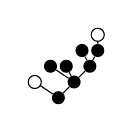
\begin{tikzpicture}[scale=.13333]
          \node[circle, scale=0.5, fill] (tid0) at (4.5,1.5){};
          \node[circle, scale=0.5, fill, task_scheduled] (tid2) at (2.25,3){};
          \node[circle, scale=0.5, fill] (tid3) at (6,3){};
          \node[circle, scale=0.5, fill] (tid5) at (3.75,4.5){};
          \node[circle, scale=0.5, fill] (tid6) at (5.25,4.5){};
          \node[circle, scale=0.5, fill] (tid7) at (7.5,4.5){};
          \node[circle, scale=0.5, fill] (tid8) at (6.75,6){};
          \node[circle, scale=0.5, fill] (tid9) at (8.25,6){};
          \node[circle, scale=0.5, fill, task_scheduled] (tid10) at (8.25,7.5){};
          \draw[](tid9) -- (tid10);
          \draw[](tid7) -- (tid8);
          \draw[](tid7) -- (tid9);
          \draw[](tid3) -- (tid5);
          \draw[](tid3) -- (tid6);
          \draw[](tid3) -- (tid7);
          \draw[](tid0) -- (tid2);
          \draw[](tid0) -- (tid3);
        \end{tikzpicture}
      };
      & 
      \node[draw=black, rectangle split,  rectangle split parts=1] (sn0x17d6160){
        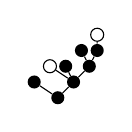
\begin{tikzpicture}[scale=.13333]
          \node[circle, scale=0.5, fill] (tid0) at (4.5,1.5){};
          \node[circle, scale=0.5, fill] (tid2) at (2.25,3){};
          \node[circle, scale=0.5, fill] (tid3) at (6,3){};
          \node[circle, scale=0.5, fill, task_scheduled] (tid5) at (3.75,4.5){};
          \node[circle, scale=0.5, fill] (tid6) at (5.25,4.5){};
          \node[circle, scale=0.5, fill] (tid7) at (7.5,4.5){};
          \node[circle, scale=0.5, fill] (tid8) at (6.75,6){};
          \node[circle, scale=0.5, fill] (tid9) at (8.25,6){};
          \node[circle, scale=0.5, fill, task_scheduled] (tid10) at (8.25,7.5){};
          \draw[](tid9) -- (tid10);
          \draw[](tid7) -- (tid8);
          \draw[](tid7) -- (tid9);
          \draw[](tid3) -- (tid5);
          \draw[](tid3) -- (tid6);
          \draw[](tid3) -- (tid7);
          \draw[](tid0) -- (tid2);
          \draw[](tid0) -- (tid3);
        \end{tikzpicture}
      };
      & 
      \node[draw=black, rectangle split,  rectangle split parts=1] (sn0x17d5380){
        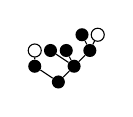
\begin{tikzpicture}[scale=.13333]
          \node[circle, scale=0.5, fill] (tid0) at (4.5,1.5){};
          \node[circle, scale=0.5, fill] (tid2) at (2.25,3){};
          \node[circle, scale=0.5, fill, task_scheduled] (tid4) at (2.25,4.5){};
          \draw[](tid2) -- (tid4);
          \node[circle, scale=0.5, fill] (tid3) at (6,3){};
          \node[circle, scale=0.5, fill] (tid5) at (3.75,4.5){};
          \node[circle, scale=0.5, fill] (tid6) at (5.25,4.5){};
          \node[circle, scale=0.5, fill] (tid7) at (7.5,4.5){};
          \node[circle, scale=0.5, fill] (tid8) at (6.75,6){};
          \node[circle, scale=0.5, fill, task_scheduled] (tid9) at (8.25,6){};
          \draw[](tid7) -- (tid8);
          \draw[](tid7) -- (tid9);
          \draw[](tid3) -- (tid5);
          \draw[](tid3) -- (tid6);
          \draw[](tid3) -- (tid7);
          \draw[](tid0) -- (tid2);
          \draw[](tid0) -- (tid3);
        \end{tikzpicture}
      };
      & 
      \node[draw=black, rectangle split,  rectangle split parts=1] (sn0x17d2f50){
        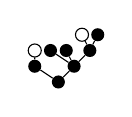
\begin{tikzpicture}[scale=.13333]
          \node[circle, scale=0.5, fill] (tid0) at (4.5,1.5){};
          \node[circle, scale=0.5, fill] (tid2) at (2.25,3){};
          \node[circle, scale=0.5, fill, task_scheduled] (tid4) at (2.25,4.5){};
          \draw[](tid2) -- (tid4);
          \node[circle, scale=0.5, fill] (tid3) at (6,3){};
          \node[circle, scale=0.5, fill] (tid5) at (3.75,4.5){};
          \node[circle, scale=0.5, fill] (tid6) at (5.25,4.5){};
          \node[circle, scale=0.5, fill] (tid7) at (7.5,4.5){};
          \node[circle, scale=0.5, fill, task_scheduled] (tid8) at (6.75,6){};
          \node[circle, scale=0.5, fill] (tid9) at (8.25,6){};
          \draw[](tid7) -- (tid8);
          \draw[](tid7) -- (tid9);
          \draw[](tid3) -- (tid5);
          \draw[](tid3) -- (tid6);
          \draw[](tid3) -- (tid7);
          \draw[](tid0) -- (tid2);
          \draw[](tid0) -- (tid3);
        \end{tikzpicture}
      };
      & 
      \node[draw=black, rectangle split,  rectangle split parts=1] (sn0x17d3a00){
        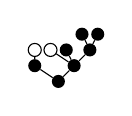
\begin{tikzpicture}[scale=.13333]
          \node[circle, scale=0.5, fill] (tid0) at (4.5,1.5){};
          \node[circle, scale=0.5, fill] (tid2) at (2.25,3){};
          \node[circle, scale=0.5, fill, task_scheduled] (tid4) at (2.25,4.5){};
          \draw[](tid2) -- (tid4);
          \node[circle, scale=0.5, fill] (tid3) at (6,3){};
          \node[circle, scale=0.5, fill, task_scheduled] (tid5) at (3.75,4.5){};
          \node[circle, scale=0.5, fill] (tid6) at (5.25,4.5){};
          \node[circle, scale=0.5, fill] (tid7) at (7.5,4.5){};
          \node[circle, scale=0.5, fill] (tid8) at (6.75,6){};
          \node[circle, scale=0.5, fill] (tid9) at (8.25,6){};
          \draw[](tid7) -- (tid8);
          \draw[](tid7) -- (tid9);
          \draw[](tid3) -- (tid5);
          \draw[](tid3) -- (tid6);
          \draw[](tid3) -- (tid7);
          \draw[](tid0) -- (tid2);
          \draw[](tid0) -- (tid3);
        \end{tikzpicture}
      };
      & 
      \\
    };
  \end{scope}
  % \draw (sn0x17d67b0.south) -- node[left, xshift=-.125cm]{$0.4$} (sn0x17d6160.north);
  % \draw (sn0x17d67b0.south) -- node[left, xshift=-.25cm]{$0.1$} (sn0x17d55b0.north);
  % \draw (sn0x17d67b0.south) -- node[right, xshift=.25]{$0.1$} (sn0x17d2f50.north);
  % \draw (sn0x17d67b0.south) -- node[left]{$0.2$} (sn0x17d5380.north);
  % \draw (sn0x17d67b0.south) -- node[right, xshift=.25cm]{$0.3$} (sn0x17d3a00.north);
  \draw (sn0x17d67b0.south) -- (sn0x17d6160.north);
  \draw (sn0x17d67b0.south) -- (sn0x17d55b0.north);
  \draw (sn0x17d67b0.south) -- (sn0x17d2f50.north);
  \draw (sn0x17d67b0.south) -- (sn0x17d5380.north);
  \draw (sn0x17d67b0.south) -- (sn0x17d3a00.north);
\end{tikzpicture}
%%% Local Variables:
%%% TeX-master: "thesis/thesis.tex"
%%% End: 

    \caption{The same snapshot DAG without intermediate snapshots. Intermediate snapshots are eliminated and the edges are drawn directly between non-intermediate snapshots. The probabilities are in shown in percent in directly within the snapshot (in the respective order). The probabilities are obtained by multiplying the corresponding probabilities along the original edges that are needed to form the new edges.}
  \label{fig:schedule-dag-intro-no-intermediates}
  \end{subfigure}
  \caption{An exemplary schedule DAG with and without intermediate snapshots. From now on, we will focus on snapshot DAGs without intermediate snapshots.}
  \label{fig:schedule-dag-intro}
\end{figure}

Figure \ref{fig:schedule-dag-intro-no-intermediates} shows the version of the schedule that omits intermediate snapshots. From now on, we will restrict ourselves to the latter structure (without intermediate snapshots) because this representation is easier to maintain and -- after some time to get accustomed to it -- as easy to understand as the version with intermediate snapshots.

\section{Computing the expected run time of a schedule}
\label{sec:introduction-compute-expected-time-schedule}

Computing the expected run time for a given schedule (more precisely for the whole processing of an intree according to a certain schedule) can be easily acchieved via a recursive formula that can be explained as follows:

\begin{itemize}
\item If the current intree $I$ consists of exactly one task (the root), then we simply have to process this single task. Since one task has expected run time $\frac{1}{\lambda}=1$ (remember: we assumed w.l.o.g $\lambda=1$), we know that the expected run time for $I$ is 1.
\item If the current intree consists of more than 1 task, there may be up to $p$ tasks scheduled, where $p$ denotes the number of processors. Let us assume that there are $r\leq p$ tasks scheduled ($r$ may be smaller than $p$ if there are less ready tasks than processors) and denote the set of these tasks by $X=\{x_1,x_2,\dots,x_r\}$. According to theorem \ref{thm:iid-cont-rand-var-minimum}, the probability that task $x_i$ ($i\in\left\{ 1,2,\dots,r \right\}$) is the \emph{first} task to finish is $\frac{1}{r}$. The expected run time for $x_i$ is $\frac{1}{n}$ (by theorems \ref{thm:minimum-of-exponential-distribution-is-exponential} and \ref{thm:exponential-distribution-expectancy}). Moreover, the probability that two tasks finish at exactly the same time is 0 (since the run times of tasks are exponentially -- i.e. continuously -- distributed).

  If task $x_i$ finishes, the remaining intree is $I\setminus\left\{ x_i \right\}$, with -- due to non-preemtive scheduling -- at least tasks within $\left\{ x_1,x_2,\dots,x_r \right\} \setminus \left\{ x_i \right\}$ scheduled. By $X_i$ we denote the set of tasks that are scheduled in the next step (i.e. $\left\{ x_1,x_2,\dots,x_r \right\} \setminus \left\{ x_i \right\} \subseteq X_i$). The expected run time for $I\setminus\left\{ x_i \right\}$ can then be computed recursively (see remark below).

  This means: If $x_i$ is the first task to finish, we can use the expected run time is given by
  \begin{equation*}
    \frac{1}{r} + T_{X_i}(I\setminus\left\{ x_i \right\}),
  \end{equation*}
  where $\frac{1}{r}$ accounts for the expected run time of task $x_i$ and $T_{X_i}(I\setminus\left\{ x_i \right\})$ denotes the run time for the intree $I\setminus\left\{ x_i \right\}$ if the tasks within $X_i$ are scheduled (of course with respect to a specific scheduling strategy).

  We define events $F_1,\dots,F_r$, where $F_i$ describes the event that task $x_i$ is the first task to finish. Note that the events $F_i$ are pairwise disjoint, $\p{F_i}=\frac{1}{r}$ and that one of the events $F_i$ \emph{must} occur (meaning that $\p{F_1\cup \dots \cup F_r}=1$).
  
  Since \emph{each} of the tasks $x_1,x_2,\dots,x_r$ can be the first task to finish (each with probability $\frac{1}{r}$ according to theorem \ref{thm:iid-cont-rand-var-minimum}), we can use theorem \ref{theo:law-total-expectation} and compute the overal run time by 
  \begin{eqnarray}
    %\nonumber
    \label{eqn:intro-recursive-formula-for-run-time-total-exp}
    \E{T_X(I)}
    &=& 
    \sum_{i=1}^r \p{F_i} \cdot \E{T_{X} (I) \mid F_i}
    = \\
    &=& 
    \label{eqn:intro-recursive-formula-for-intermediate-form}
    \sum_{i=1}^r \p{F_i} \cdot \E{T(x_i) + T_{X_i} (I \setminus \{x_i\})}
    = \\
    \label{eqn:intro-recursive-formula-for-intermediate-form-2}
    &=& \sum_{i=1}^r \frac{1}{r} \cdot \left( \frac{1}{r} + \E{T_{X_i}\left( I\setminus\left\{ x_i \right\} \right)} \right) = \\
    \label{eqn:intro-recursive-formula-for-run-time}
    &=&     
    \frac{1}{r} + \frac{1}{r} \cdot \sum_{i=1}^r \E{T_{X_i}\left( I\setminus\left\{ x_i \right\} \right)}.
  \end{eqnarray}
\end{itemize}

\emph{Remark:} We can reformulate (\ref{eqn:intro-recursive-formula-for-run-time-total-exp}) to (\ref{eqn:intro-recursive-formula-for-intermediate-form}) because the expected run time to process the whole tree $I$ under the condition $F_i$ (i.e. under the knowledge that task $x_i$ is the first to finish) can be computed by summing up the time that is needed by task $x_i$ (thus the term $T(x_i)$) and the time needed for the remaining tree (denoted by $T_{X_i}(I)\setminus\{x_i\}$).

Since all tasks' processing times are assumed to be exponentially distributed, i.e. in particular memoryless (see theorem \ref{thm:exponential-memoryless}), we can argue as follows: If one task finishes, the other scheduled tasks -- of course -- \emph{might} have been processed up to a certain point. But since their processing times are memoryless, we can assume them to behave \emph{as if} they had not been processed at all. That is, the remaining tree can be considered \emph{as if} we just started all scheduled tasks. This, however, means that we are in the same situation as before, except that we are dealing with an intree that has one task less than the intree before. Thus, we can justify the reformulation from (\ref{eqn:intro-recursive-formula-for-intermediate-form}) to (\ref{eqn:intro-recursive-formula-for-intermediate-form-2}).

%The fact that we can compute the expected run time \emph{recursively} follows from the fact that exponentially distributed random variables are memoryless (see theorem \ref{thm:exponential-memoryless}): 


As an example, consider the tree in figure \ref{fig:intro-computing-expected-runtime}. The topmost snapshots describe the first step of schedules for three resp. four processors on the same intree. We are the corresponding expected run times. We can assume that the run times of the snapshots in the second line have already been computed (recursively). Using these, we can compute the overal expected run time using theorem (\ref{eqn:intro-recursive-formula-for-run-time}) as described in figures \ref{fig:intro-recursive-formula-run-time-example-three-procs} and \ref{fig:intro-recursive-formula-run-time-example-four-procs}. 

\begin{figure}[tt]
  \centering
  \begin{subfigure}{.45\textwidth}
    \renewcommand{\leveltopI}{-15cm + \leveltop}
    \renewcommand{\leveltopII}{-15cm + \leveltopI}
    \renewcommand{\leveltopIII}{-15cm + \leveltopII}
    \centering
    \begin{tikzpicture}[scale=.2, anchor=south]
      \begin{scope}[yshift=\leveltopI cm]
        \matrix (line1)[column sep=.5cm] {
          \node[draw=black, rectangle split,  rectangle split parts=2] (sn0x834df78){
            \begin{tikzpicture}[scale=.2]
              \node[circle, scale=0.75, fill] (tid0) at (3,1.5){};
              \node[circle, scale=0.75, fill] (tid1) at (2.25,3){};
              \node[circle, scale=0.75, fill, task_scheduled] (tid2) at (0.75,4.5){};
              \node[circle, scale=0.75, fill] (tid4) at (3,4.5){};
              \node[circle, scale=0.75, fill] (tid5) at (2.25,6){};
              \node[circle, scale=0.75, fill] (tid7) at (2.25,7.5){};
              \node[circle, scale=0.75, fill, task_scheduled] (tid8) at (2.25,9){};
              \draw[](tid7) -- (tid8);
              \draw[](tid5) -- (tid7);
              \node[circle, scale=0.75, fill, task_scheduled] (tid6) at (3.75,6){};
              \draw[](tid4) -- (tid5);
              \draw[](tid4) -- (tid6);
              \draw[](tid1) -- (tid2);
              \draw[](tid1) -- (tid4);
              \node[circle, scale=0.75, fill] (tid3) at (5.25,3){};
              \draw[](tid0) -- (tid1);
              \draw[](tid0) -- (tid3);
            \end{tikzpicture}
            \nodepart{two}
            \footnotesize{6.21811}
          };
          & 
          \\
        };
      \end{scope}
      \begin{scope}[yshift=\leveltopII cm]
        \matrix (line2)[column sep=.5cm] {
          \node[draw=black, rectangle split,  rectangle split parts=2] (sn0x834f4d0){
            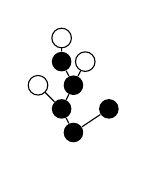
\begin{tikzpicture}[scale=.2]
              \node[circle, scale=0.75, fill] (tid0) at (3,1.5){};
              \node[circle, scale=0.75, fill] (tid1) at (2.25,3){};
              \node[circle, scale=0.75, fill, task_scheduled] (tid2) at (0.75,4.5){};
              \node[circle, scale=0.75, fill] (tid4) at (3,4.5){};
              \node[circle, scale=0.75, fill] (tid5) at (2.25,6){};
              \node[circle, scale=0.75, fill, task_scheduled] (tid7) at (2.25,7.5){};
              \draw[](tid5) -- (tid7);
              \node[circle, scale=0.75, fill, task_scheduled] (tid6) at (3.75,6){};
              \draw[](tid4) -- (tid5);
              \draw[](tid4) -- (tid6);
              \draw[](tid1) -- (tid2);
              \draw[](tid1) -- (tid4);
              \node[circle, scale=0.75, fill] (tid3) at (5.25,3){};
              \draw[](tid0) -- (tid1);
              \draw[](tid0) -- (tid3);
            \end{tikzpicture}
            \nodepart{two}
            \footnotesize{5.41204}
          };
          & 
          \node[draw=black, rectangle split,  rectangle split parts=2] (sn0x834ec08){
            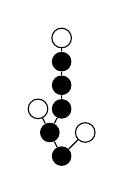
\begin{tikzpicture}[scale=.2]
              \node[circle, scale=0.75, fill] (tid0) at (2.25,1.5){};
              \node[circle, scale=0.75, fill] (tid1) at (1.5,3){};
              \node[circle, scale=0.75, fill, task_scheduled] (tid2) at (0.75,4.5){};
              \node[circle, scale=0.75, fill] (tid4) at (2.25,4.5){};
              \node[circle, scale=0.75, fill] (tid5) at (2.25,6){};
              \node[circle, scale=0.75, fill] (tid7) at (2.25,7.5){};
              \node[circle, scale=0.75, fill, task_scheduled] (tid8) at (2.25,9){};
              \draw[](tid7) -- (tid8);
              \draw[](tid5) -- (tid7);
              \draw[](tid4) -- (tid5);
              \draw[](tid1) -- (tid2);
              \draw[](tid1) -- (tid4);
              \node[circle, scale=0.75, fill, task_scheduled] (tid3) at (3.75,3){};
              \draw[](tid0) -- (tid1);
              \draw[](tid0) -- (tid3);
            \end{tikzpicture}
            \nodepart{two}
            \footnotesize{6.09066}
          };
          & 
          \node[draw=black, rectangle split,  rectangle split parts=2] (sn0x834f908){
            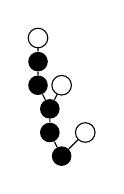
\begin{tikzpicture}[scale=.2]
              \node[circle, scale=0.75, fill] (tid0) at (2.25,1.5){};
              \node[circle, scale=0.75, fill] (tid1) at (1.5,3){};
              \node[circle, scale=0.75, fill] (tid4) at (1.5,4.5){};
              \node[circle, scale=0.75, fill] (tid5) at (0.75,6){};
              \node[circle, scale=0.75, fill] (tid7) at (0.75,7.5){};
              \node[circle, scale=0.75, fill, task_scheduled] (tid8) at (0.75,9){};
              \draw[](tid7) -- (tid8);
              \draw[](tid5) -- (tid7);
              \node[circle, scale=0.75, fill, task_scheduled] (tid6) at (2.25,6){};
              \draw[](tid4) -- (tid5);
              \draw[](tid4) -- (tid6);
              \draw[](tid1) -- (tid4);
              \node[circle, scale=0.75, fill, task_scheduled] (tid3) at (3.75,3){};
              \draw[](tid0) -- (tid1);
              \draw[](tid0) -- (tid3);
            \end{tikzpicture}
            \nodepart{two}
            \footnotesize{6.15162}
          };
          & 
          \\
        };
      \end{scope}
      \draw (sn0x834df78.south) -- (sn0x834f4d0.north);
      \draw (sn0x834df78.south) -- (sn0x834ec08.north);
      \draw (sn0x834df78.south) -- (sn0x834f908.north);
    \end{tikzpicture}
    \caption{Three processors. 
      Transition probabilities are $\frac{1}{3}$ each.
      Then, we can compute $
      \frac{1}{3}+\frac{1}{3}\cdot
      \left( 
        5.41204 + 6.09066 + 6.15162
      \right)
      = 6.21811$.
    }
    \label{fig:intro-recursive-formula-run-time-example-three-procs}
  \end{subfigure}
  \quad
  \begin{subfigure}{.45\textwidth}
    \centering
    \renewcommand{\leveltopI}{-15cm + \leveltop}
    \renewcommand{\leveltopII}{-15cm + \leveltopI}
    \renewcommand{\leveltopIII}{-15cm + \leveltopII}
    \renewcommand{\leveltopIIII}{-15cm + \leveltopIII}
    \renewcommand{\leveltopIIIII}{-15cm + \leveltopIIII}
    \renewcommand{\leveltopIIIIII}{-15cm + \leveltopIIIII}
    \renewcommand{\leveltopIIIIIII}{-15cm + \leveltopIIIIII}
    \renewcommand{\leveltopIIIIIIII}{-15cm + \leveltopIIIIIII}
    \renewcommand{\leveltopIIIIIIIII}{-15cm + \leveltopIIIIIIII}
    \begin{tikzpicture}[scale=.2, anchor=south]
      \begin{scope}[yshift=\leveltopI cm]
        \matrix (line1)[column sep=.5cm] {
          \node[draw=black, rectangle split,  rectangle split parts=2] (sn0x9500f78){
            \begin{tikzpicture}[scale=.2]
              \node[circle, scale=0.75, fill] (tid0) at (3,1.5){};
              \node[circle, scale=0.75, fill] (tid1) at (2.25,3){};
              \node[circle, scale=0.75, fill, task_scheduled] (tid2) at (0.75,4.5){};
              \node[circle, scale=0.75, fill] (tid4) at (3,4.5){};
              \node[circle, scale=0.75, fill] (tid5) at (2.25,6){};
              \node[circle, scale=0.75, fill] (tid7) at (2.25,7.5){};
              \node[circle, scale=0.75, fill, task_scheduled] (tid8) at (2.25,9){};
              \draw[](tid7) -- (tid8);
              \draw[](tid5) -- (tid7);
              \node[circle, scale=0.75, fill, task_scheduled] (tid6) at (3.75,6){};
              \draw[](tid4) -- (tid5);
              \draw[](tid4) -- (tid6);
              \draw[](tid1) -- (tid2);
              \draw[](tid1) -- (tid4);
              \node[circle, scale=0.75, fill, task_scheduled] (tid3) at (5.25,3){};
              \draw[](tid0) -- (tid1);
              \draw[](tid0) -- (tid3);
            \end{tikzpicture}
            \nodepart{two}
            \footnotesize{6.20264}
          };
          & 
          \\
        };
      \end{scope}
      \begin{scope}[yshift=\leveltopII cm]
        \matrix (line2)[column sep=.5cm] {
          \node[draw=black, rectangle split,  rectangle split parts=2] (sn0x9502500){
            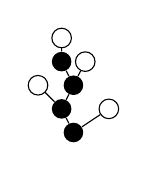
\begin{tikzpicture}[scale=.2]
              \node[circle, scale=0.75, fill] (tid0) at (3,1.5){};
              \node[circle, scale=0.75, fill] (tid1) at (2.25,3){};
              \node[circle, scale=0.75, fill, task_scheduled] (tid2) at (0.75,4.5){};
              \node[circle, scale=0.75, fill] (tid4) at (3,4.5){};
              \node[circle, scale=0.75, fill] (tid5) at (2.25,6){};
              \node[circle, scale=0.75, fill, task_scheduled] (tid7) at (2.25,7.5){};
              \draw[](tid5) -- (tid7);
              \node[circle, scale=0.75, fill, task_scheduled] (tid6) at (3.75,6){};
              \draw[](tid4) -- (tid5);
              \draw[](tid4) -- (tid6);
              \draw[](tid1) -- (tid2);
              \draw[](tid1) -- (tid4);
              \node[circle, scale=0.75, fill, task_scheduled] (tid3) at (5.25,3){};
              \draw[](tid0) -- (tid1);
              \draw[](tid0) -- (tid3);
            \end{tikzpicture}
            \nodepart{two}
            \footnotesize{5.39005}
          };
          & 
          \node[draw=black, rectangle split,  rectangle split parts=2] (sn0x9501c08){
            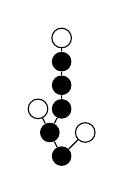
\begin{tikzpicture}[scale=.2]
              \node[circle, scale=0.75, fill] (tid0) at (2.25,1.5){};
              \node[circle, scale=0.75, fill] (tid1) at (1.5,3){};
              \node[circle, scale=0.75, fill, task_scheduled] (tid2) at (0.75,4.5){};
              \node[circle, scale=0.75, fill] (tid4) at (2.25,4.5){};
              \node[circle, scale=0.75, fill] (tid5) at (2.25,6){};
              \node[circle, scale=0.75, fill] (tid7) at (2.25,7.5){};
              \node[circle, scale=0.75, fill, task_scheduled] (tid8) at (2.25,9){};
              \draw[](tid7) -- (tid8);
              \draw[](tid5) -- (tid7);
              \draw[](tid4) -- (tid5);
              \draw[](tid1) -- (tid2);
              \draw[](tid1) -- (tid4);
              \node[circle, scale=0.75, fill, task_scheduled] (tid3) at (3.75,3){};
              \draw[](tid0) -- (tid1);
              \draw[](tid0) -- (tid3);
            \end{tikzpicture}
            \nodepart{two}
            \footnotesize{6.09066}
          };
          & 
          \node[draw=black, rectangle split,  rectangle split parts=2] (sn0x95028b8){
            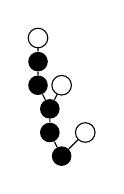
\begin{tikzpicture}[scale=.2]
              \node[circle, scale=0.75, fill] (tid0) at (2.25,1.5){};
              \node[circle, scale=0.75, fill] (tid1) at (1.5,3){};
              \node[circle, scale=0.75, fill] (tid4) at (1.5,4.5){};
              \node[circle, scale=0.75, fill] (tid5) at (0.75,6){};
              \node[circle, scale=0.75, fill] (tid7) at (0.75,7.5){};
              \node[circle, scale=0.75, fill, task_scheduled] (tid8) at (0.75,9){};
              \draw[](tid7) -- (tid8);
              \draw[](tid5) -- (tid7);
              \node[circle, scale=0.75, fill, task_scheduled] (tid6) at (2.25,6){};
              \draw[](tid4) -- (tid5);
              \draw[](tid4) -- (tid6);
              \draw[](tid1) -- (tid4);
              \node[circle, scale=0.75, fill, task_scheduled] (tid3) at (3.75,3){};
              \draw[](tid0) -- (tid1);
              \draw[](tid0) -- (tid3);
            \end{tikzpicture}
            \nodepart{two}
            \footnotesize{6.15162}
          };
          & 
          \node[draw=black, rectangle split,  rectangle split parts=2] (sn0x9502a20){
            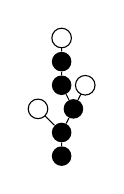
\begin{tikzpicture}[scale=.2]
              \node[circle, scale=0.75, fill] (tid0) at (2.25,1.5){};
              \node[circle, scale=0.75, fill] (tid1) at (2.25,3){};
              \node[circle, scale=0.75, fill, task_scheduled] (tid2) at (0.75,4.5){};
              \node[circle, scale=0.75, fill] (tid4) at (3,4.5){};
              \node[circle, scale=0.75, fill] (tid5) at (2.25,6){};
              \node[circle, scale=0.75, fill] (tid7) at (2.25,7.5){};
              \node[circle, scale=0.75, fill, task_scheduled] (tid8) at (2.25,9){};
              \draw[](tid7) -- (tid8);
              \draw[](tid5) -- (tid7);
              \node[circle, scale=0.75, fill, task_scheduled] (tid6) at (3.75,6){};
              \draw[](tid4) -- (tid5);
              \draw[](tid4) -- (tid6);
              \draw[](tid1) -- (tid2);
              \draw[](tid1) -- (tid4);
              \draw[](tid0) -- (tid1);
            \end{tikzpicture}
            \nodepart{two}
            \footnotesize{6.17824}
          };
          & 
          \\
        };
      \end{scope}
      \draw (sn0x9500f78.south) -- (sn0x9502500.north);
      \draw (sn0x9500f78.south) -- (sn0x9501c08.north);
      \draw (sn0x9500f78.south) -- (sn0x95028b8.north);
      \draw (sn0x9500f78.south) -- (sn0x9502a20.north);
    \end{tikzpicture}
    \caption{Four processors. Transition probabilities between snapshots are $\frac{1}{4}$ each, so we can compute the overal expected run time by 
      $
      \frac{1}{4} + \frac{1}{4}\cdot 
      \left( 
        5.39005 + 6.09066 + 6.15162 + 6.17824
      \right)
      = 6.20264
      $
    }
    \label{fig:intro-recursive-formula-run-time-example-four-procs}
  \end{subfigure}
  \caption{Computing the expected run time according to equation (\ref{eqn:intro-recursive-formula-for-run-time}) for three resp. four processors on the same intree. Each box represents a single snapshot containing the intree (with scheduled tasks marked) and the expected run time for the respective snapshot.}
  \label{fig:intro-computing-expected-runtime}
\end{figure}

\paragraph{Computing the runtime for an in-forset}

As mentioned in section \ref{sec:intrees-extension-to-forests}, we can also deal with in-forests by adding a new root connected to all intrees of the forest. To compute the expected run time for a specific schedule, we simply compute the expected run time for the intree resulting from the in-forest conversion and subtract 1. This can be done because the last task in the resulting intree to be processed \emph{must} be the root we introduced. The expected run time for the root is 1, so we can simply subtract 1 to obtain the expected run time for the original in-forest.

\section{Optimizing a given schedule}
\label{sec:algorithm-computing-optimal-schedule}

Now we know how to compute a schedule according to a specific scheduling strategy. We now describe an algorithm that can be used to improve the original schedule. It recursively discards ``wrong choices'', i.e. decisions that are suboptimal. The technique for it is shown in algorithm \ref{alg:optimize-snapshot}.

\begin{algorithm}[t]
  \begin{algorithmic}[5]
    \Procedure{OptimizeSnapshot}{$s$}
      \Comment{$s$ is the snapshot to be optimized}
    \For{$t \in scheduled(s)$}
      \Comment{Iterate over all currently scheduled tasks}
    \State $sucs_t \gets \left\{ s' \mid s' \text{ is a successor of } s \text{ resulting if } t \text{ is the first finishing task} \right\}$
    \State $osucs_t \gets \left\{ \Call{OptimizeSnapshot}{s'} \mid s' \in sucs_t \right\}$
    \EndFor
    \State $\displaystyle newsucs \gets \bigcup_{t\in scheduled(s)}  \Call{BestSnaps}{osucs_t} $
    \State \textbf{return} new snapshot with successors $newsucs$ and adjusted transition probabilities
    \label{alg:optimize-snap-adjust-probs}
    \EndProcedure
    \Statex
    \Procedure{BestSnaps}{$snaps$}
      \State \textbf{return} $\left\{ s \mid s\in snaps, expectedTime(s) \leq \min\left\{ expectedTime(s')\mid s' \in snaps \right\} \right\}$
    \EndProcedure
  \end{algorithmic}
  \caption{Optimizing a given shapshot recursively}
  \label{alg:optimize-snapshot}
\end{algorithm}

Line \ref{alg:optimize-snap-adjust-probs} of algorithm \ref{alg:optimize-snapshot} needs some explanation: We did not in particular specify how to ``adjust'' the probabilities properly. This is because there are different solutions. The only thing that must be kept in mind is that the sum of all probabilities for reaching a snapshot from the set $\Call{BestSnaps}{osucs_t}$ must be equal to the probability that task $t$ is the first task to finish (i.e. in our particular case, it must be equal to $\frac{1}{r}$ if there are $r$ tasks scheduled for the respective snapshot).

One canonical way of assigning probabilities to snapshots within $\Call{BestSnaps}{osucs_t}$ is to assign probability $\frac{1}{r\cdot|\Call{BestSnaps}{osucs_t}|}$ to each of the snapshots within this set. Another way is to choose one particular element in $\Call{BestSnaps}{osucs_t}$ and assign it probability $\frac{1}{r}$ while all other snapshots in $\Call{BestSnaps}{osucs_t}$ get probability 0. This way, we eliminate further snapshots by making them impossible to reach. The latter method is especially useful because it automatically eliminates some snapshots that are not needed.

An important aspect of this optimization routine is that we can -- in an implementation -- assure that it is executed \emph{at most once} for each snapshot (by simply having a flag that indicates whether a snapshot was already subject to optimization). This means that we can assure that the total cost to optimize all snapshots of a schedule is bounded by $O\left(\sum_{s\in D} optcost(s)\right)$ where $D$ denotes the snapshot DAG for the particular scheduler and $optcost(s)$ gives the cost to optimize a snapshot $s$. If we know the most expensive snapshot to optimize and call it $s^*$ we can argue that $O\left(\sum_{s\in D} optcost(s)\right) \subseteq O\left(|D|\cdot optcost(s^*)\right)$.

\section{Computing the optimal schedule}
\label{sec:intro-computing-optimal-schedule}

We saw that we can optimize a given schedule and exploit this fact in conjunction with the LEAF scheduler (that corresponds to an exhaustive search). We first compute \emph{all possible} schedules using the LEAF scheduler and -- afterwards -- optimize this using algorithm \ref{alg:optimize-snapshot}. This way, we can compute the optimal schedule by an exhaustive search.

It is clear that the resulting schedule must be optimal because algorithm \ref{alg:optimize-snapshot} chooses -- for each scheduled task $t$ that could be the first to finish -- only the best solutions. Since a ``complete schedule'' from the LEAF schedule contains all possible schedules as a part of it, the optimization algorithm picks the best choices possible for each step.

Again, we can give the asymptotic run time of $O\left(|D| \cdot optcost(s^*)\right)$ (see section \ref{sec:algorithm-computing-optimal-schedule}), and we can tell that the snapshot DAG $D$ for an intree $I$ scheduled on $p$ processors contains \emph{at most} $| \left\{ T \mid T\subseteq I \right\} | \cdot n^p$ snapshots. This can be easily explained because each snapshot is associated with a subtree of $I$ and for this subtree we have at most $n^p$ possible choices for the tasks to be scheduled. Note that in practice there are much less snapshots than this given bound because e.g. it is in most cases not possible to have $n^p$ combinations for the scheduled tasks.

\section{Equivalent snapshots}
\label{sec:intro-first-glance-schedules}

We now move on to describing a basic insight about schedules. Foremost, we make the following -- quite simple -- observation: If two intrees $I_1$ and $I_2$ are isomorphic, then for each schedule $S_1$ for $I_1$, there is a schedule $S_2$ for $I_2$ that has exactly the same run time. We see this by examining the bijective function $f:I_1 \mapsto I_2$ and for $S_2$ scheduling exactly the task $f(t_1)$ if $S_1$ would choose $t_1$.

The second observation is that we can make the snapshot DAG more compact by avoiding snapshots that are -- essentially -- duplicates. We therefore extend the concept of isomorphisms from trees to snapshots in a straightforward way.

\begin{definition}[Equivalent snapshots]
  Let $S=(I, X)$ be a snapshot with intree $I$ and a set $X$ of currently scheduled tasks. The snapshot $S'=(I', X')$ is called \emph{equivalent} to $S$ if there is an intree isomorphism from $I$ onto $I'$ such that the sets of scheduled tasks also correspond under this isomorhpsim 
  (i.e. $X' = \left\{ f(x) \mid x\in X \right\}$).

  If $S$ and $S'$ are not equivalent, we call them \emph{distinct}.
\end{definition}

The requirement that scheduled tasks are ``preserved'' by the isomorphism is central to equivalence of snapshots, because otherwise, the corresponding run times may be unequal. Figure \ref{fig:non-isomorphic-snapshots} shows two variants of the intree $(0,0,0,1,1)$ with different sets of scheduled tasks, resulting in two distinct snapshots.

\begin{figure}
  \centering
  \begin{subfigure}{.45\textwidth}
    \centering
    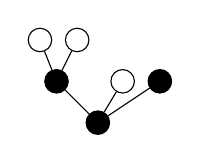
\begin{tikzpicture}[scale=.35]
      \node[circle, scale=0.9, fill, draw=black] (tid0) at (3,1.5){};
      \node[circle, scale=0.9, fill, draw=black] (tid1) at (1.5,3){};
      \node[circle, scale=0.9, fill, task_scheduled] (tid4) at (0.9,4.5){};
      \node[circle, scale=0.9, fill, task_scheduled] (tid6) at (2.25,4.5){};
      \draw[](tid1) -- (tid4);
      \draw[](tid1) -- (tid6);
      \node[circle, scale=0.9, fill, task_scheduled] (tid3) at (3.9,3){};
      \node[circle, scale=0.9, fill, draw=black] (tid5) at (5.25,3){};
      \draw[](tid0) -- (tid1);
      \draw[](tid0) -- (tid3);
      \draw[](tid0) -- (tid5);
    \end{tikzpicture}
    \caption{Intree $(0,0,0,1,1)$ with scheduled tasks 2, 4 and 5.}
  \end{subfigure}
  \quad
  \begin{subfigure}{.45\textwidth}
    \centering
    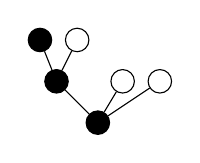
\begin{tikzpicture}[scale=.35]
      \node[circle, scale=0.9, fill, draw=black] (tid0) at (3,1.5){};
      \node[circle, scale=0.9, fill, draw=black] (tid1) at (1.5,3){};
      \node[circle, scale=0.9, fill, draw=black] (tid4) at (0.9,4.5){};
      \node[circle, scale=0.9, fill, task_scheduled] (tid6) at (2.25,4.5){};
      \draw[](tid1) -- (tid4);
      \draw[](tid1) -- (tid6);
      \node[circle, scale=0.9, fill, task_scheduled] (tid3) at (3.9,3){};
      \node[circle, scale=0.9, fill, task_scheduled] (tid5) at (5.25,3){};
      \draw[](tid0) -- (tid1);
      \draw[](tid0) -- (tid3);
      \draw[](tid0) -- (tid5);
    \end{tikzpicture}
    \caption{Intree $(0,0,0,1,1)$ with scheduled tasks 2, 3 and 5.}
  \end{subfigure}
  \caption{Two non-equivalent (i.e. \emph{distinct}) snapshots. This example shows that even if the underlying intrees are isomorphic, the containing snapshots are not necessarily equivalent, because there is no isomorphism between the two intrees that preserves scheduled tasks.}
  \label{fig:non-isomorphic-snapshots}
\end{figure}

It can be easily seen that we essentially compute the same thing twice if we carry out computations for several equivalent snapshots. Therefore, we can combine equivalent snapshots into one snapshot. This transformation (treating equivalent snapshots as one single snapshot) requires us to adjust the probabilities in the snapshot DAG, which can be done straightforward by summing up all probabilities along the edges that are merged into one single edge. Figure \ref{fig:intro-equivalent-snapshots-elimination} shows an example where we would originally have to deal with six snapshots, but can reduce this to only two snapshots by excluding equivalent snapshots.

\begin{figure}[tt]
  \centering
  \renewcommand{\leveltopI}{-10cm + \leveltop}
  \renewcommand{\leveltopII}{-10cm + \leveltopI}
  \begin{subfigure}{\textwidth}
    \centering{}
    \begin{tikzpicture}[scale=.35, anchor=south]
      \node[text width=4cm](info) at (14,-10){Each transition shown has a probability of $\frac{1}{6}$.};
      \draw[->, dashed] (info) ..controls+(0,-2)and+(+2,0).. +(-5,-5);
      \draw[->, dashed] (info) ..controls+(0,-2)and+(+2,0).. +(-11,-5);
      \tikzstyle{task_scheduled}=[fill=white, draw]
      \begin{scope}[yshift=\leveltopI cm]
        \matrix (line1)[column sep=0.25cm] {
          \node[draw=black, rectangle split,  rectangle split parts=1] (sn0x9bc9928){
            \begin{tikzpicture}[scale=.35]
              \node[circle, scale=0.75, fill=white!80!black, draw=black] (tid0) at (3.75,1.5){\scriptsize{0}};
              \node[circle, scale=0.75, fill=white!80!black, draw=black] (tid1) at (1.5,3){\scriptsize{1}};
              \node[circle, scale=0.75, fill, task_scheduled] (tid4) at (0.75,4.5){\scriptsize{4}};
              \node[circle, scale=0.75, fill, task_scheduled] (tid6) at (2.25,4.5){\scriptsize{6}};
              \draw[](tid1) -- (tid4);
              \draw[](tid1) -- (tid6);
              \node[circle, scale=0.75, fill, task_scheduled] (tid2) at (3.75,3){\scriptsize{2}};
              \node[circle, scale=0.75, fill=white!80!black, draw=black] (tid3) at (5.25,3){\scriptsize{3}};
              \node[circle, scale=0.75, fill=white!80!black, draw=black] (tid5) at (6.75,3){\scriptsize{5}};
              \draw[](tid0) -- (tid1);
              \draw[](tid0) -- (tid2);
              \draw[](tid0) -- (tid3);
              \draw[](tid0) -- (tid5);
            \end{tikzpicture}
          };
          & 
          \\
        };
      \end{scope}
      \begin{scope}[yshift=\leveltopII cm]
        \matrix (line2)[column sep=0.25cm] {
          \node[draw=black, rectangle split,  rectangle split parts=1] (sn0x9bcb370){
            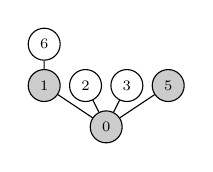
\begin{tikzpicture}[scale=.35]
              \node[circle, scale=0.75, fill=white!80!black, draw=black] (tid0) at (3,1.5){\scriptsize{0}};
              \node[circle, scale=0.75, fill=white!80!black, draw=black] (tid1) at (0.75,3){\scriptsize{1}};
              \node[circle, scale=0.75, fill, task_scheduled] (tid6) at (0.75,4.5){\scriptsize{6}};
              \draw[](tid1) -- (tid6);
              \node[circle, scale=0.75, fill, task_scheduled] (tid2) at (2.25,3){\scriptsize{2}};
              \node[circle, scale=0.75, fill, task_scheduled] (tid3) at (3.75,3){\scriptsize{3}};
              \node[circle, scale=0.75, fill=white!80!black, draw=black] (tid5) at (5.25,3){\scriptsize{5}};
              \draw[](tid0) -- (tid1);
              \draw[](tid0) -- (tid2);
              \draw[](tid0) -- (tid3);
              \draw[](tid0) -- (tid5);
            \end{tikzpicture}
          };
          & 
          \node[draw=black, rectangle split,  rectangle split parts=1] (sn0x9bd1828){
            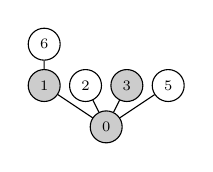
\begin{tikzpicture}[scale=.35]
              \node[circle, scale=0.75, fill=white!80!black, draw=black] (tid0) at (3,1.5){\scriptsize{0}};
              \node[circle, scale=0.75, fill=white!80!black, draw=black] (tid1) at (0.75,3){\scriptsize{1}};
              \node[circle, scale=0.75, fill, task_scheduled] (tid6) at (0.75,4.5){\scriptsize{6}};
              \draw[](tid1) -- (tid6);
              \node[circle, scale=0.75, fill, task_scheduled] (tid2) at (2.25,3){\scriptsize{2}};
              \node[circle, scale=0.75, fill=white!80!black, draw=black] (tid3) at (3.75,3){\scriptsize{3}};
              \node[circle, scale=0.75, fill, task_scheduled] (tid5) at (5.25,3){\scriptsize{5}};
              \draw[](tid0) -- (tid1);
              \draw[](tid0) -- (tid2);
              \draw[](tid0) -- (tid3);
              \draw[](tid0) -- (tid5);
            \end{tikzpicture}
          };
          & 
          \node[draw=black, rectangle split,  rectangle split parts=1] (sn0x9bd0f28){
            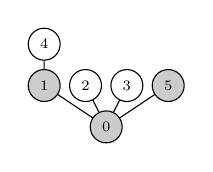
\begin{tikzpicture}[scale=.35]
              \node[circle, scale=0.75, fill=white!80!black, draw=black] (tid0) at (3,1.5){\scriptsize{0}};
              \node[circle, scale=0.75, fill=white!80!black, draw=black] (tid1) at (0.75,3){\scriptsize{1}};
              \node[circle, scale=0.75, fill, task_scheduled] (tid4) at (0.75,4.5){\scriptsize{4}};
              \draw[](tid1) -- (tid4);
              \node[circle, scale=0.75, fill, task_scheduled] (tid2) at (2.25,3){\scriptsize{2}};
              \node[circle, scale=0.75, fill, task_scheduled] (tid3) at (3.75,3){\scriptsize{3}};
              \node[circle, scale=0.75, fill=white!80!black, draw=black] (tid5) at (5.25,3){\scriptsize{5}};
              \draw[](tid0) -- (tid1);
              \draw[](tid0) -- (tid2);
              \draw[](tid0) -- (tid3);
              \draw[](tid0) -- (tid5);
            \end{tikzpicture}
          };
          & 
          \node[draw=black, rectangle split,  rectangle split parts=1] (sn0x9bd2140){
            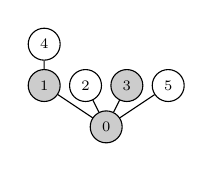
\begin{tikzpicture}[scale=.35]
              \node[circle, scale=0.75, fill=white!80!black, draw=black] (tid0) at (3,1.5){\scriptsize{0}};
              \node[circle, scale=0.75, fill=white!80!black, draw=black] (tid1) at (0.75,3){\scriptsize{1}};
              \node[circle, scale=0.75, fill, task_scheduled] (tid4) at (0.75,4.5){\scriptsize{4}};
              \draw[](tid1) -- (tid4);
              \node[circle, scale=0.75, fill, task_scheduled] (tid2) at (2.25,3){\scriptsize{2}};
              \node[circle, scale=0.75, fill=white!80!black, draw=black] (tid3) at (3.75,3){\scriptsize{3}};
              \node[circle, scale=0.75, fill, task_scheduled] (tid5) at (5.25,3){\scriptsize{5}};
              \draw[](tid0) -- (tid1);
              \draw[](tid0) -- (tid2);
              \draw[](tid0) -- (tid3);
              \draw[](tid0) -- (tid5);
            \end{tikzpicture}
          };
          & 
          \node[draw=black, rectangle split,  rectangle split parts=1] (sn0x9bc7440){
            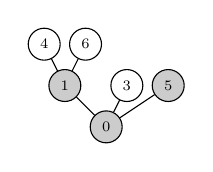
\begin{tikzpicture}[scale=.35]
              \node[circle, scale=0.75, fill=white!80!black, draw=black] (tid0) at (3,1.5){\scriptsize{0}};
              \node[circle, scale=0.75, fill=white!80!black, draw=black] (tid1) at (1.5,3){\scriptsize{1}};
              \node[circle, scale=0.75, fill, task_scheduled] (tid4) at (0.75,4.5){\scriptsize{4}};
              \node[circle, scale=0.75, fill, task_scheduled] (tid6) at (2.25,4.5){\scriptsize{6}};
              \draw[](tid1) -- (tid4);
              \draw[](tid1) -- (tid6);
              \node[circle, scale=0.75, fill, task_scheduled] (tid3) at (3.75,3){\scriptsize{3}};
              \node[circle, scale=0.75, fill=white!80!black, draw=black] (tid5) at (5.25,3){\scriptsize{5}};
              \draw[](tid0) -- (tid1);
              \draw[](tid0) -- (tid3);
              \draw[](tid0) -- (tid5);
            \end{tikzpicture}
          };
          & 
          \node[draw=black, rectangle split,  rectangle split parts=1] (sn0x9bd1530){
            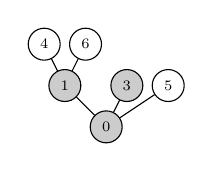
\begin{tikzpicture}[scale=.35]
              \node[circle, scale=0.75, fill=white!80!black, draw=black] (tid0) at (3,1.5){\scriptsize{0}};
              \node[circle, scale=0.75, fill=white!80!black, draw=black] (tid1) at (1.5,3){\scriptsize{1}};
              \node[circle, scale=0.75, fill, task_scheduled] (tid4) at (0.75,4.5){\scriptsize{4}};
              \node[circle, scale=0.75, fill, task_scheduled] (tid6) at (2.25,4.5){\scriptsize{6}};
              \draw[](tid1) -- (tid4);
              \draw[](tid1) -- (tid6);
              \node[circle, scale=0.75, fill=white!80!black, draw=black] (tid3) at (3.75,3){\scriptsize{3}};
              \node[circle, scale=0.75, fill, task_scheduled] (tid5) at (5.25,3){\scriptsize{5}};
              \draw[](tid0) -- (tid1);
              \draw[](tid0) -- (tid3);
              \draw[](tid0) -- (tid5);
            \end{tikzpicture}
          };
          & 
          \\
        };
      \end{scope}
      \draw (sn0x9bc9928.south) -- (sn0x9bc7440.north);
      \draw (sn0x9bc9928.south) -- (sn0x9bd1530.north);
      \draw (sn0x9bc9928.south) -- (sn0x9bcb370.north);
      \draw (sn0x9bc9928.south) -- (sn0x9bd1828.north);
      \draw (sn0x9bc9928.south) -- (sn0x9bd0f28.north);
      \draw (sn0x9bc9928.south) -- (sn0x9bd2140.north);
      \begin{scope}[yshift=-3cm]
        \draw[decorate,decoration={brace,mirror}] (-22,-17)
        --node[below, yshift=-.1cm]{Task 4 finished first} +(14.1,0);
        \draw[decorate,decoration={brace,mirror}] (-7.4,-17)
        --node[below, yshift=-.1cm]{Task 6 finished first} +(14.1,0);
        \draw[decorate,decoration={brace,mirror}] (7.2,-17)
        --node[below, yshift=-.1cm]{Task 2 finished first} +(14.1,0);
        % equivalences
        \draw[decorate,decoration={brace,mirror}] (-22,-19)
        --node[below, yshift=-.1cm]{4 equivalent snapshots} +(28.5,0);
        \draw[decorate,decoration={brace,mirror}] (7.2,-19)
        --node[below, yshift=-.1cm]{2 equivalent snapshots} +(14.1,0);
      \end{scope}
    \end{tikzpicture}
    \caption{Schedule DAG showing all possible snapshots. Tasks currently scheduled are drawn white. Other tasks are drawn gray.}
  \end{subfigure}
  \begin{subfigure}{\textwidth}
    \renewcommand{\leveltopII}{-10cm + \leveltopI}
    \centering{}
    \begin{tikzpicture}[scale=.2, anchor=south]
      \begin{scope}[yshift=\leveltopI cm]
        \matrix (line1)[column sep=0.25cm] {
          \node[draw=black, rectangle split,  rectangle split parts=1] (sn0x9bc9928){
            \begin{tikzpicture}[scale=.2]
              \node[circle, scale=0.75, fill, draw=black] (tid0) at (3.75,1.5){};
              \node[circle, scale=0.75, fill, draw=black] (tid1) at (1.5,3){};
              \node[circle, scale=0.75, fill, task_scheduled] (tid4) at (0.75,4.5){};
              \node[circle, scale=0.75, fill, task_scheduled] (tid6) at (2.25,4.5){};
              \draw[](tid1) -- (tid4);
              \draw[](tid1) -- (tid6);
              \node[circle, scale=0.75, fill, task_scheduled] (tid2) at (3.75,3){};
              \node[circle, scale=0.75, fill, draw=black] (tid3) at (5.25,3){};
              \node[circle, scale=0.75, fill, draw=black] (tid5) at (6.75,3){};
              \draw[](tid0) -- (tid1);
              \draw[](tid0) -- (tid2);
              \draw[](tid0) -- (tid3);
              \draw[](tid0) -- (tid5);
            \end{tikzpicture}
          };
          & 
          \\
        };
      \end{scope}
      \begin{scope}[yshift=\leveltopII cm]
        \matrix (line2)[column sep=0.25cm] {
          \node[draw=black, rectangle split,  rectangle split parts=1] (sn0x9bd2140){
            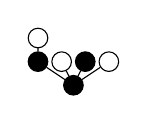
\begin{tikzpicture}[scale=.2]
              \node[circle, scale=0.75, fill, draw=black] (tid0) at (3,1.5){};
              \node[circle, scale=0.75, fill, draw=black] (tid1) at (0.75,3){};
              \node[circle, scale=0.75, fill, task_scheduled] (tid4) at (0.75,4.5){};
              \draw[](tid1) -- (tid4);
              \node[circle, scale=0.75, fill, task_scheduled] (tid2) at (2.25,3){};
              \node[circle, scale=0.75, fill, draw=black] (tid3) at (3.75,3){};
              \node[circle, scale=0.75, fill, task_scheduled] (tid5) at (5.25,3){};
              \draw[](tid0) -- (tid1);
              \draw[](tid0) -- (tid2);
              \draw[](tid0) -- (tid3);
              \draw[](tid0) -- (tid5);
            \end{tikzpicture}
          };
          & 
          \node[draw=black, rectangle split,  rectangle split parts=1] (sn0x9bc7440){
            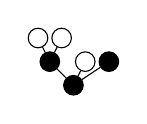
\begin{tikzpicture}[scale=.2]
              \node[circle, scale=0.75, fill, draw=black] (tid0) at (3,1.5){};
              \node[circle, scale=0.75, fill, draw=black] (tid1) at (1.5,3){};
              \node[circle, scale=0.75, fill, task_scheduled] (tid4) at (0.75,4.5){};
              \node[circle, scale=0.75, fill, task_scheduled] (tid6) at (2.25,4.5){};
              \draw[](tid1) -- (tid4);
              \draw[](tid1) -- (tid6);
              \node[circle, scale=0.75, fill, task_scheduled] (tid3) at (3.75,3){};
              \node[circle, scale=0.75, fill, draw=black] (tid5) at (5.25,3){};
              \draw[](tid0) -- (tid1);
              \draw[](tid0) -- (tid3);
              \draw[](tid0) -- (tid5);
            \end{tikzpicture}
          };
          & 
          \\
        };
      \end{scope}
      \draw[] (sn0x9bc9928.south) --node[right,xshift=.1cm]{$\frac{2}{6}$} (sn0x9bc7440.north);
      \draw[] (sn0x9bc9928.south) --node[left,xshift=-.1cm]{$\frac{4}{6}$} (sn0x9bd2140.north);
    \end{tikzpicture}
    \caption{Condensed DAG with distinct snapshots only.}
  \end{subfigure}
  \quad
  \caption{Equivalent snapshots can be eliminated. Note that this changes the probabilities along the edges. To obtain the new probabilities, we sum up the probabilities all edges that are merged into the corresponding edge.}
  \label{fig:intro-equivalent-snapshots-elimination}
\end{figure}

From now on, if not stated otherwise, we restrict ourselves to snapshot DAGs that contain only distinct snapshots.

\section{Snapshot DAGs revisited}
\label{sec:introduction-snapshot-dags-revisited}

We have seen transition probabilities between certain snapshots, how compute the expected run time of a schedule recursively, excluding equivalent snapshots. We now come back to the description of a schedule as a snapshot DAG (as introduced in section \ref{sec:intro-visualizing-schedules}) that already contained the transition probabilities as elements in the corresponding snapshots.

We augment this visualization by two new elements: The expected run time for a snapshot and probability of reaching a certain snapshot.

\begin{figure}[th]
  \centering
  \renewcommand{\leveltopI}{-13cm + \leveltop}
\renewcommand{\leveltopII}{-13cm + \leveltopI}
\renewcommand{\leveltopIII}{-15cm + \leveltopII}
\renewcommand{\leveltopIIII}{-13cm + \leveltopIII}
\renewcommand{\leveltopIIIII}{-12cm + \leveltopIIII}
\renewcommand{\leveltopIIIIII}{-10cm + \leveltopIIIII}
\begin{tikzpicture}[scale=.2, anchor=south]
\begin{scope}[yshift=\leveltopI cm]
\matrix (line1)[column sep=1cm] {
\node[draw=black, rectangle split,  rectangle split parts=4] (sn0x9434200){
\footnotesize{100}
\nodepart{two}
\begin{tikzpicture}[scale=.2]
\node[circle, scale=0.75, fill] (tid0) at (2.25,1.5){};
\node[circle, scale=0.75, fill] (tid1) at (1.5,3){};
\node[circle, scale=0.75, fill, task_scheduled] (tid3) at (0.75,4.5){};
\node[circle, scale=0.75, fill, task_scheduled] (tid4) at (2.25,4.5){};
\draw[](tid1) -- (tid3);
\draw[](tid1) -- (tid4);
\node[circle, scale=0.75, fill] (tid2) at (3.75,3){};
\node[circle, scale=0.75, fill, task_scheduled] (tid5) at (3.75,4.5){};
\draw[](tid2) -- (tid5);
\draw[](tid0) -- (tid1);
\draw[](tid0) -- (tid2);
\end{tikzpicture}
\nodepart{three}
\footnotesize{4.05556}
\nodepart{four}
\footnotesize{$33\:67$}
};
 & 
\\
};
\end{scope}
\begin{scope}[yshift=\leveltopII cm]
\matrix (line2)[column sep=1cm] {
\node[draw=black, rectangle split,  rectangle split parts=4] (sn0x9432698){
\footnotesize{33.3333}
\nodepart{two}
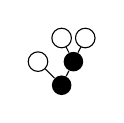
\begin{tikzpicture}[scale=.2]
\node[circle, scale=0.75, fill] (tid0) at (2.25,1.5){};
\node[circle, scale=0.75, fill, task_scheduled] (tid1) at (0.75,3){};
\node[circle, scale=0.75, fill] (tid2) at (3,3){};
\node[circle, scale=0.75, fill, task_scheduled] (tid3) at (2.25,4.5){};
\node[circle, scale=0.75, fill, task_scheduled] (tid4) at (3.75,4.5){};
\draw[](tid2) -- (tid3);
\draw[](tid2) -- (tid4);
\draw[](tid0) -- (tid1);
\draw[](tid0) -- (tid2);
\end{tikzpicture}
\nodepart{three}
\footnotesize{3.66667}
\nodepart{four}
\footnotesize{$67\:33$}
};
 & 
\node[draw=black, rectangle split,  rectangle split parts=4] (sn0x94339c8){
\footnotesize{66.6667}
\nodepart{two}
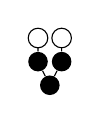
\begin{tikzpicture}[scale=.2]
\node[circle, scale=0.75, fill] (tid0) at (1.5,1.5){};
\node[circle, scale=0.75, fill] (tid1) at (0.75,3){};
\node[circle, scale=0.75, fill, task_scheduled] (tid3) at (0.75,4.5){};
\draw[](tid1) -- (tid3);
\node[circle, scale=0.75, fill] (tid2) at (2.25,3){};
\node[circle, scale=0.75, fill, task_scheduled] (tid4) at (2.25,4.5){};
\draw[](tid2) -- (tid4);
\draw[](tid0) -- (tid1);
\draw[](tid0) -- (tid2);
\end{tikzpicture}
\nodepart{three}
\footnotesize{3.75}
\nodepart{four}
\footnotesize{$100$}
};
 & 
\\
};
\end{scope}
\begin{scope}[yshift=\leveltopIII cm]
\matrix (line3)[column sep=1cm] {
\node[draw=black, rectangle split,  rectangle split parts=4] (sn0x9432e80){
\footnotesize{88.8889}
\nodepart{two}
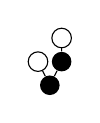
\begin{tikzpicture}[scale=.2]
\node[circle, scale=0.75, fill] (tid0) at (1.5,1.5){};
\node[circle, scale=0.75, fill, task_scheduled] (tid1) at (0.75,3){};
\node[circle, scale=0.75, fill] (tid2) at (2.25,3){};
\node[circle, scale=0.75, fill, task_scheduled] (tid3) at (2.25,4.5){};
\draw[](tid2) -- (tid3);
\draw[](tid0) -- (tid1);
\draw[](tid0) -- (tid2);
\end{tikzpicture}
\nodepart{three}
\footnotesize{3.25}
\nodepart{four}
\footnotesize{$50\:50$}
};
 & 
\node[draw=black, rectangle split,  rectangle split parts=4] (sn0x94332c8){
\footnotesize{11.1111}
\nodepart{two}
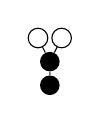
\begin{tikzpicture}[scale=.2]
\node[circle, scale=0.75, fill] (tid0) at (1.5,1.5){};
\node[circle, scale=0.75, fill] (tid1) at (1.5,3){};
\node[circle, scale=0.75, fill, task_scheduled] (tid2) at (0.75,4.5){};
\node[circle, scale=0.75, fill, task_scheduled] (tid3) at (2.25,4.5){};
\draw[](tid1) -- (tid2);
\draw[](tid1) -- (tid3);
\draw[](tid0) -- (tid1);
\end{tikzpicture}
\nodepart{three}
\footnotesize{3.5}
\nodepart{four}
\footnotesize{$100$}
};
 & 
\\
};
\end{scope}
\begin{scope}[yshift=\leveltopIIII cm]
\matrix (line4)[column sep=1cm] {
\node[draw=black, rectangle split,  rectangle split parts=4] (sn0x9433530){
\footnotesize{44.4444}
\nodepart{two}

\begin{tikzpicture}[scale=.2]
\node[circle, scale=0.75, fill] (tid0) at (1.5,1.5){};
\node[circle, scale=0.75, fill, task_scheduled] (tid1) at (0.75,3){};
\node[circle, scale=0.75, fill, task_scheduled] (tid2) at (2.25,3){};
\draw[](tid0) -- (tid1);
\draw[](tid0) -- (tid2);
\end{tikzpicture}
\nodepart{three}
\footnotesize{2.5}
\nodepart{four}
\footnotesize{$100$}
};
 & 
\node[draw=black, rectangle split,  rectangle split parts=4] (sn0x9432888){
\footnotesize{55.5556}
\nodepart{two}
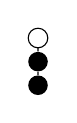
\begin{tikzpicture}[scale=.2]
\node[circle, scale=0.75, fill] (tid0) at (0.75,1.5){};
\node[circle, scale=0.75, fill] (tid1) at (0.75,3){};
\node[circle, scale=0.75, fill, task_scheduled] (tid2) at (0.75,4.5){};
\draw[](tid1) -- (tid2);
\draw[](tid0) -- (tid1);
\end{tikzpicture}
\nodepart{three}
\footnotesize{3}
\nodepart{four}
\footnotesize{$100$}
};
 & 
\\
};
\end{scope}
\begin{scope}[yshift=\leveltopIIIII cm]
\matrix (line5)[column sep=1cm] {
\node[draw=black, rectangle split,  rectangle split parts=4] (sn0x9431fb8){
\footnotesize{100}
\nodepart{two}
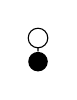
\begin{tikzpicture}[scale=.2]
\node[circle, scale=0.75, fill] (tid0) at (0.75,1.5){};
\node[circle, scale=0.75, fill, task_scheduled] (tid1) at (0.75,3){};
\draw[](tid0) -- (tid1);
\end{tikzpicture}
\nodepart{three}
\footnotesize{2}
\nodepart{four}
\footnotesize{$100$}
};
 & 
\\
};
\end{scope}
\begin{scope}[yshift=\leveltopIIIIII cm]
\matrix (line6)[column sep=1cm] {
\node[draw=black, rectangle split,  rectangle split parts=4] (sn0x9432988){
\footnotesize{100}
\nodepart{two}

\begin{tikzpicture}[scale=.2]
\node[circle, scale=0.75, fill, task_scheduled] (tid0) at (0.75,1.5){};
\end{tikzpicture}
\nodepart{three}
\footnotesize{1}
\nodepart{four}
\footnotesize{$$}
};
 & 
\\
};
\end{scope}
\draw (sn0x9434200.south) -- (sn0x94339c8.north);
\draw (sn0x9434200.south) -- (sn0x9432698.north);
\draw (sn0x9432698.south) -- (sn0x94332c8.north);
\draw (sn0x9432698.south) -- (sn0x9432e80.north);
\draw (sn0x94339c8.south) -- (sn0x9432e80.north);
\draw (sn0x9432e80.south) -- (sn0x9432888.north);
\draw (sn0x9432e80.south) -- (sn0x9433530.north);
\draw (sn0x94332c8.south) -- (sn0x9432888.north);
\draw (sn0x9433530.south) -- (sn0x9431fb8.north);
\draw (sn0x9432888.south) -- (sn0x9431fb8.north);
\draw (sn0x9431fb8.south) -- (sn0x9432988.north);
\end{tikzpicture}
%%% Local Variables:
%%% TeX-master: "thesis/thesis.tex"
%%% End: 

  \caption{Snapshot DAG with each node containing the following elements of the respective snapshot: Probability of reaching it, intree (with scheduled tasks marked), expected run time, probability of successors.}
  \label{fig:intro-complete-dag}
\end{figure}

Figure \ref{fig:intro-complete-dag} visualizes a schedule for the intree $(0,0,1,1,2)$ processed by three processors. This snapshot DAG contains -- for each snapshot -- the probability of reaching it, the corresponding intree, the expected run time and the probabilities for the successors.

\section{Summary: Problem statement}
\label{sec:introduction-aim}

We now sum up what we have as input and what we want to do:
\begin{itemize}
\item Given an intree of tasks,\dots
\item \dots whose run times are independently, identically exponentially distributed, \dots
\item \dots and that can not be preemted \dots
\item \dots we want to obtain an optimal scheduling strategy, \dots
\item in the sense that we want to minimize the overal expected run time.
\end{itemize}

There is a convenient and de-facto standard notation for scheduling problems (see \cite{schedulingclassification}) that basically consists of three fields $\alpha$, $\beta$ and $\gamma$ separated by a vertical bar. We do not go into details about this notation, but we will briefly characterize our problem under consideration in this notation.

The first part, $\alpha$, describes the \emph{machine environment}. We assume that we have a set of identical machines which is indicated by $\alpha = P$. Because we are mainly dealing with 2 or 3 identical machines, we can be more concrete and set $\alpha = P2$ resp. $\alpha=P3$.

After we have specified the machine environment, we now describe the \emph{job characteristics} with the symbol $\beta$. The field $\beta$ that can be seen to consist of several parts $\beta_1,\beta_2,\dots$, of which we concentrate on the most important ones:

\begin{itemize}
\item We are mainly interested in a scenario where jobs can not be preemted, i.e. once a job is assigned it has to be processed until the end. Using the notation from \cite{schedulingclassification} this is indicated by leaving $\beta_1$ empty.
\item As said, we are dealing with intrees, this is -- in \cite{schedulingclassification} -- denoted by $\beta_3=tree$. To emphasize that we are dealing with \emph{intrees} (in contrast to \emph{outtrees}), we set $\beta_3=intree$.
\item We are dealing with tasks whose processing times are not known a priori but are assumed to behave like  independent exponentially distributed variables with same parameters. This notation is not intended by \cite{schedulingclassification} which is why we introduce a new notation by $\beta_7 = exp$.
\end{itemize}

The fields of $\beta$ that we did not mention here are left empty.

In total, we have $\beta = intree, exp$ indicating that we have an intree structure of tasks whose processing times are assumed to be random variables as described.

Last, we specify the \emph{optimality criteria} resp. the \emph{objective} we want to acchieve. As said we are interested in keeping the expected overal run time low. The notation from \cite{schedulingclassification} is not designed for stochastic scheduling problems, which is why we extend the notaion to incorporate the \emph{expected makespan}. Following \cite{pinedo2008scheduling} we could simply write $\gamma = C_{max}$ but to emphasize that we are talking about the \emph{expected} makespan, we will set $\gamma = \E{C_{max}}$.

To sum up, we consider the scheduling problems described by
\begin{equation*}
  P2 \mid intree, exp \mid \E{C_{max}} 
  \quad \text{ and } \quad
  P3 \mid intree, exp \mid \E{C_{max}}
  .
\end{equation*}


%%% Local Variables:
%%% TeX-master: "../thesis.tex"
%%% End: 